\section{Ein neues Projekt erstellen}
Um eine Aufnahme machen zu können, müssen wir zuerst ein neues Projekt erstellen. Startet dazu Traverso und wählt im Menü ,,Projekt $\rightarrow$ Neu\dots''. Gebt dem Projekt einen Namen, setzt die Anzahl Seiten auf 1, und die Anzahl Spuren auf 2. Lasst die restlichen Felder leer. Dann klickt ,,OK'' um das neue Projekt zu laden. Alle aufgenommenen Audiodateien werden übrigens in \texttt{projekt-verzeichnis/projekt-name/audiosources} gespeichert. Wenn ihr also unserem Rat gefolgt seid und das Projektverzeichnis auf einer Partition mit viel freiem Speicherplatz angelegt habt, solltet ihr im Folgenden keine Probleme aufgrund von zu wenig Speicherplatz haben.

\section{Den Treiber einrichten}
Sollte der Treiber noch nicht eingerichtet sein, öffnet nun den Einstellungsdialog im Menü ,,Einstellungen $\rightarrow$ Einstellungen\dots''. Weitere Details zum einrichten des Treibers findet man in Kapitel \ref{sect_setup}. In diesen Einstellungen kann auch die Sample-Frequenz eingestellt werden, mit der Traverso die Hardware anspricht. Das Dateiformat für die aufgenommenen Audiodateien kann im Menu ,,Einstellungen $\rightarrow$ Format der Aufnahmedateien'' ausgewählt werden. Die Signalauflösung beträgt durchgängig 32 Bit, deshalb verwendet Traverso unabhängig von Format und Treibereinstellung 32 Bit Fliesskomma-Auflösung zum speichern der Audiodaten.

\section{Die Aufnahme}
Stellt sicher dass ein Signal am Eingangskanal der Soundkarte anliegt, z.\,B. ein CD-Player der abspielt. Drückt \sact{B} auf dem ersten Kanal in Traverso und wählt ,,Capture 1'' als Eingangskanal. Dann drückt \sact{A} um die erste Spur für die Aufnahme zu aktivieren. Sobald der Aufnahmemodus aktiv ist, sollte im VUMeter das Eingangssignal angezeigt werden. Ist dies nicht der Fall, so ist vermutlich das Problem au"serhalb von Traverso zu suchen. Überprüft ob wirklich ein Gerät an Line-In angeschlossen ist, und dass es auch wirklich abspielt. Dann öffnet ein Mixerprogramm wi zum Beispiel KMix, mit dem ihr eure Soundkarte konfigurieren könnt. Es kann zum Beispiel sein, dass die Eingangskanäle stummgeschaltet sind und erst aktiviert werden müssen (\FigB\ \ref{fig_kmix01}).

\begin{figure}
 \centering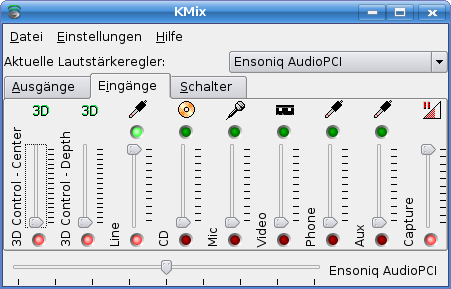
\includegraphics[width=0.8\textwidth]{../images/kmix01.png}
 \caption{Mit KMix kann die Soundkarte konfiguriert werden. Stellt sicher dass die Eingangskanäle nicht stummgeschaltet sind (Line und Capture) und für die Aufnahme aktiviert wurden (grüne und rote Knöpfe).}
 \label{fig_kmix01}
\end{figure}

Wenn alles für die Aufnahme bereit ist, drückt den \texttt{Aufnahme}-Knopf in der Titelleiste oder STRG+\sact{Leertaste} um die Aufnahme zu starten. Mit \sact{Leertaste} wird sie wieder gestoppt. Das war's auch schon. Um die Aufnahme anzuhören platziert den Arbeitscursor vor dem neuen Clip, drückt \sact{V} und startet das Abspielen mit \sact{Leertaste}. Vergesst nicht nach der Aufnahme den Record-Modus der Spuren wieder zu deaktivieren indem ihr \sact{A} auf den aktiven Spuren drückt, oder \dact{A} um alle aktiven Spuren gleichzeitig zu deaktivieren.
